\chapter{Rétrosynthèse et stratégie de synthèse multiétape}\label{ch:b2:retrosynthesis}

Une molécule est dessinée au tableau, et personne ne sait encore comment la préparer. Essayer des
réactions dans le sens direct, à partir de ce qui se trouve sur l'étagère, ne mène nulle part~: il y en
a trop. Le chimiste procède dans l'autre sens, de la cible vers l'étagère, en coupant sur le papier une
liaison à la fois, chaque coupure défaisant une réaction dont on sait qu'elle fonctionne, jusqu'à ce que
les fragments soient des composés que l'on peut acheter. Ce chapitre transforme les réactions des
chapitres précédents en ce raisonnement à rebours, puis se demande comment juger la voie qu'il produit.

\begin{recall}
Du \cref{ch:b2:alkene-redox} au \cref{ch:b2:wittig}~: les réactions à défaire. Le volume de première
année~: groupes protecteurs et acétals, organomagnésiens et inversion de polarité, synthèse de
Williamson, chimiosélectivité, oxydation des alcools. Le volume scolaire~: économie d'atomes.
\end{recall}

\section{Raisonner à rebours}

\begin{definition}[Analyse rétrosynthétique]\label{def:b2:retrosynthesis:analysis}
La molécule à préparer est la \emph{molécule cible}\index{molecule cible@molécule cible}. L'\emph{analyse
rétrosynthétique}\index{analyse retrosynthetique@analyse rétrosynthétique} remonte de la cible vers des
produits de départ disponibles,
par étapes dont chacune est l'inverse d'une réaction connue~; une étape rétrosynthétique s'écrit avec la
flèche double $\Rightarrow$, qui se lit «~est préparé à partir de~».
\end{definition}

\begin{definition}[Déconnexion et synthons]\label{def:b2:retrosynthesis:disconnection}
Une \emph{déconnexion}\index{deconnexion@déconnexion} est la coupure imaginaire d'une liaison de la
cible, l'inverse d'une réaction qui forme une liaison. Couper une liaison de façon hétérolytique donne
deux \emph{synthons}\index{synthon}, fragments chargés idéalisés, l'un donneur (nucléophile, souvent
négatif), l'autre accepteur (électrophile, souvent positif). Un \emph{équivalent synthétique}\index{equivalent synthetique@équivalent synthétique}
est un réactif réel qui se comporte comme un synthon~: un organomagnésien pour le carbanion \ce{R-}, un
aldéhyde pour le cation $\mathrm{R\overset{+}{C}H{-}OH}$.
\end{definition}

\begin{definition}[Interconversion de groupe fonctionnel]\label{def:b2:retrosynthesis:fgi}
Une \emph{interconversion de groupe fonctionnel}\index{interconversion de groupe fonctionnel} (IGF)
est une étape rétrosynthétique qui modifie un groupe fonctionnel sans changer le squelette carboné~: un
alcool à partir d'une cétone (par réduction), une chaîne alcane à partir d'un alcène (par
hydrogénation), une amine à partir d'un amide.
\end{definition}

\begin{omfigure}
\begin{tikzpicture}[every node/.style={align=center}]
\node (T) at (0,0) {\setchemfig{atom sep=1.7em}\chemfig{Ph-CH(-[2]OH)-CH(-[6]CH_3)-CH_3}};
\node (A) at (-4.6,-2.6) {\ce{PhCHO}\\[1pt] + \ce{(CH3)2CHMgBr}};
\node (B) at (0,-2.6) {\ce{PhMgBr}\\[1pt] + \ce{(CH3)2CHCHO}};
\node (C) at (4.6,-2.6) {\setchemfig{atom sep=1.7em}\chemfig{Ph-C(=[2]O)-CH(-[6]CH_3)-CH_3}};
\node (D) at (4.6,-5.0) {\ce{C6H6}\\[1pt] + \ce{(CH3)2CHCOCl}};
\draw[omretro] (T.south west) -- node[above left, font=\small] {a} (A.north);
\draw[omretro] (T.south) -- node[right, font=\small] {b} (B.north);
\draw[omretro] (T.south east) -- node[above right, font=\small] {IGF} (C.north);
\draw[omretro] (C.south) -- node[right, font=\small] {c} (D.north);
\end{tikzpicture}
\par\vspace{6pt}

{\small Un arbre rétrosynthétique pour le 2-méthyl-1-phénylpropan-1-ol. (a) et (b)~: les deux
\omterm{def:b2:retrosynthesis:disconnection}{déconnexions} de la liaison \ce{C-C} voisine du carbone de l'alcool, chacune donnant un aldéhyde et un
organomagnésien. IGF~: l'alcool à partir d'une cétone, par réduction~; (c) la cétone par \omterm{def:b2:aromatic-substitution:friedel-crafts}{acylation de
Friedel--Crafts} du benzène. Chaque flèche se lit «~est préparé à partir de~».}
\end{omfigure}

L'arbre montre les habitudes de la méthode. On choisit une \omterm{def:b2:retrosynthesis:disconnection}{déconnexion} au niveau d'une liaison voisine
d'un groupe fonctionnel, parce que c'est là que les réactions forment des liaisons. Chaque coupure est
vérifiée en écrivant les \omterm{def:b2:retrosynthesis:disconnection}{synthons} et en leur trouvant des réactifs réels. Et il y a rarement une seule
réponse~: l'arbre se ramifie, et les branches sont jugées à la fin (\cref{sec:b2:retrosynthesis:judging}).

\begin{omfigure}
\begin{center}
\small
\renewcommand{\arraystretch}{1.25}
\begin{tabular}{lll}
\hline
\omterm{def:b2:retrosynthesis:disconnection}{Synthon} & Type & \omterm{def:b2:retrosynthesis:disconnection}{Équivalent synthétique} \\
\hline
\ce{R-} (alkyle, aryle) & donneur & \ce{RMgBr}, \ce{RLi}, \ce{R2CuLi} (conjuguée) \\
$\mathrm{^-CH_2COR}$ & donneur & l'\omterm{def:b2:enolates-aldol:enolate}{énolate} de \ce{CH3COR}, ou le 3-oxobutanoate d'éthyle \\
$\mathrm{^-C{\equiv}N}$ & donneur & \ce{NaCN} \\
$\mathrm{R\overset{+}{C}H{-}OH}$ & accepteur & l'aldéhyde \ce{RCHO} \\
$\mathrm{R\overset{+}{C}{=}O}$ & accepteur & le \omterm{def:b2:acyl-substitution:derivative}{chlorure d'acyle} \ce{RCOCl}, un ester \\
\ce{R+} (primaire) & accepteur & l'halogénure \ce{RBr} (substitution bimoléculaire) \\
$\mathrm{^+CH_2CH_2COR}$ & accepteur & l'énone \ce{CH2=CHCOR} (\omterm{def:b2:conjugate-additions:addition-modes}{addition conjuguée}) \\
\hline
\end{tabular}
\end{center}

{\small \omterm{def:b2:retrosynthesis:disconnection}{Synthons} courants et leurs \omterm{def:b2:retrosynthesis:disconnection}{équivalents synthétiques}. Les \omterm{def:b2:retrosynthesis:disconnection}{synthons} donneurs sont des carbanions,
les \omterm{def:b2:retrosynthesis:disconnection}{synthons} accepteurs des carbocations~; les réactifs réels portent la même polarité sans la charge entière.}
\end{omfigure}

\section{Déconnexions à un groupe}

Une \omterm{def:b2:retrosynthesis:disconnection}{déconnexion} à un groupe coupe une liaison voisine d'un seul groupe fonctionnel. Pour une liaison
\ce{C-O} ou \ce{C-N} d'un éther, d'un ester ou d'une amine, la coupure passe entre le carbone et
l'hétéroatome~: l'hétéroatome est le donneur, le carbone l'accepteur (une synthèse de Williamson, une
\omterm{def:b2:acyl-substitution:esterification}{estérification}, une formation d'amide). Pour une liaison \ce{C-C}, le groupe fonctionnel fixe la
polarité des \omterm{def:b2:retrosynthesis:disconnection}{synthons}~: à côté d'un carbone d'alcool, ce carbone est l'accepteur (un aldéhyde ou une
cétone) et l'autre carbone le donneur (un organométallique)~; à côté d'un carbonyle, le carbone $\alpha$
est le donneur (un \omterm{def:b2:enolates-aldol:enolate}{énolate}).

La plupart de ces réactions exigent le bon niveau d'oxydation au bon endroit, si bien que les IGF entre
niveaux d'oxydation sont les étapes les plus courantes d'une voie~: alcène, alcool, aldéhyde ou cétone,
acide. L'une d'elles est restée en suspens dans le volume de première année~: arrêter l'oxydation d'un
alcool primaire à l'aldéhyde.

\begin{proposition}[Oxydations ménagées]\label{prop:b2:retrosynthesis:mild-oxidation}
Un alcool primaire est oxydé en aldéhyde, sans aller jusqu'à l'acide, par un oxydant utilisé dans un
solvant organique anhydre~: le chlorochromate de pyridinium dans le dichlorométhane, l'oxydation de
Swern (diméthylsulfoxyde activé par le chlorure d'oxalyle, puis triéthylamine, à basse température) ou
le périodinane de Dess--Martin. Dans l'eau, le chrome(VI) ou le permanganate l'oxydent en acide carboxylique.
\end{proposition}

\begin{proof}[Argument]
Ces oxydants arrachent l'hydrogène de la liaison \ce{C-H} portée par le carbone qui porte un \ce{OH}.
L'aldéhyde formé n'a plus de tel groupe. Dans l'eau, en revanche, un aldéhyde est en équilibre avec son
hydrate \ce{RCH(OH)2}, qui porte de nouveau un \ce{OH} sur un carbone porteur d'un hydrogène~: l'hydrate
est oxydé comme un alcool, jusqu'à l'acide. Sans eau, aucun hydrate ne se forme, et l'oxydation s'arrête
à l'aldéhyde.
\end{proof}

\section{Déconnexions à deux groupes}

Quand la cible porte deux groupes fonctionnels, la meilleure \omterm{def:b2:retrosynthesis:disconnection}{déconnexion} les utilise en général tous
les deux~: la liaison est coupée de sorte que l'un des groupes oriente le donneur et l'autre
l'accepteur. La distance entre les groupes, comptée en carbones d'un carbone fonctionnalisé à l'autre
bornes comprises, indique la réaction à utiliser.

\begin{proposition}[Motifs et réactions]\label{prop:b2:retrosynthesis:patterns}
Les relations entre deux groupes correspondent comme suit aux réactions des chapitres précédents. Les
relations impaires (1,3 et 1,5) correspondent aux polarités naturelles de la chimie des carbonyles~; les
relations paires (1,4 et 1,6) non, et exigent une inversion de polarité ou la coupure d'un cycle.
\end{proposition}


\begin{proof}[Argument]
En chimie des carbonyles, le carbone du carbonyle est un accepteur et le carbone $\alpha$ un donneur, et
une énone ajoute un accepteur sur son carbone $\beta$. Un \omterm{def:b2:enolates-aldol:enolate}{énolate} (donneur en $\alpha$) sur un carbonyle
(accepteur sur le carbone du carbonyle) relie les carbones 1 et 2 d'un motif 1,3~: \omterm{def:b2:enolates-aldol:aldol}{aldolisation} et
Claisen. Un \omterm{def:b2:enolates-aldol:enolate}{énolate} sur le carbone $\beta$ d'une énone construit un motif 1,5~: Michael, puis Robinson.
Pour un motif 1,4, la coupure laisse un carbone $\alpha$ comme accepteur~; aucun réactif carbonylé
ordinaire n'offre cette polarité, mais une $\alpha$-bromocétone l'offre, puisque le bromure est un groupe
partant sur ce carbone. Un composé 1,6-dicarbonylé est un cyclohexène ouvert par \omterm{def:b2:alkene-redox:cleavage}{ozonolyse}
(\cref{prop:b2:alkene-redox:ozonolysis}), et le cyclohexène se prépare par une \omterm{def:b2:frontier-orbitals:diels-alder}{réaction de Diels--Alder}
(\cref{def:b2:frontier-orbitals:diels-alder}).
\end{proof}

\begin{omfigure}
\begin{center}
\small
\renewcommand{\arraystretch}{1.25}
\begin{tabular}{lll}
\hline
Motif dans la cible & \omterm{def:b2:retrosynthesis:disconnection}{Déconnexion} & Réaction \\
$\beta$-hydroxycarbonylé (1,3) & liaison $\alpha$--$\beta$ & \omterm{def:b2:enolates-aldol:aldol}{aldolisation} \\
carbonylé $\alpha,\beta$-insaturé & \ce{C=C} & \omterm{def:b2:enolates-aldol:aldol}{crotonisation} \\
1,3-dicarbonylé & C(O)--C$\alpha$ & \omterm{def:b2:enolates-aldol:claisen}{condensation de Claisen} \\
1,5-dicarbonylé & C$\alpha$--C$\beta$ (accepteur) & \omterm{def:b2:conjugate-additions:michael}{addition de Michael} \\
cyclohex-2-én-1-one & \ce{C=C} cyclique, puis Michael & \omterm{def:b2:conjugate-additions:robinson}{annélation de Robinson} \\
cyclohexène & deux liaisons \ce{C-C} du cycle & \omterm{def:b2:frontier-orbitals:diels-alder}{réaction de Diels--Alder} \\
alcène en position définie & \ce{C=C} & \omterm{def:b2:wittig:wittig}{réaction de Wittig} ou HWE \\
1,4-dicarbonylé & \ce{C-C} centrale & \omterm{def:b2:enolates-aldol:enolate}{énolate} + $\alpha$-halogénocétone \\
1,6-dicarbonylé & relier les extrémités & \omterm{def:b2:alkene-redox:cleavage}{coupure oxydante} d'un cyclohexène \\
\hline
\end{tabular}
\end{center}

{\small Les \omterm{def:b2:retrosynthesis:disconnection}{déconnexions} à deux groupes. Les six premières utilisent la polarité normale~: un \omterm{def:b2:enolates-aldol:enolate}{énolate}
(donneur) sur un carbonyle ou une énone (accepteur). Le motif 1,4 exige qu'un carbone en $\alpha$ d'un
carbonyle soit l'accepteur, à l'inverse de son rôle habituel, ce que fournit une $\alpha$-halogénocétone.}
\end{omfigure}

\begin{method}[Une analyse rétrosynthétique]\label{met:b2:retrosynthesis:retrosynthesis}
\begin{enumerate}
  \item Énumérer les groupes fonctionnels de la cible et leurs relations (1,2~; 1,3~; \dots).
  \item Envisager les IGF qui donneraient un motif doté d'une bonne \omterm{def:b2:retrosynthesis:disconnection}{déconnexion} (un alcool à partir d'une
        cétone, une chaîne alcane à partir d'un alcène).
  \item Choisir des liaisons stratégiques~: voisines d'un groupe fonctionnel, proches du milieu de la
        molécule, à un point de ramification ou reliant un cycle à une chaîne, de sorte que les fragments
        soient de tailles comparables.
  \item Écrire les \omterm{def:b2:retrosynthesis:disconnection}{synthons}, puis leurs \omterm{def:b2:retrosynthesis:disconnection}{équivalents synthétiques}~; rejeter une coupure sans réactif réel.
  \item Vérifier la chimiosélectivité~: quel autre groupe réagirait avec chaque réactif~? Prévoir une
        protection ou changer l'ordre des étapes.
  \item Recommencer sur chaque fragment jusqu'à ce que tous soient disponibles~; écrire ensuite la voie dans
        le sens direct, avec réactifs et conditions.
\end{enumerate}
\end{method}

\section{Les groupes protecteurs dans une voie de synthèse}

Une voie exige souvent un réactif qui attaquerait un second groupe de la molécule. Le volume de première
année a protégé les aldéhydes et les cétones sous forme d'acétals. Une voie choisit parmi plusieurs
groupes protecteurs, chacun retiré dans ses propres conditions~: les acétals (retirés par un acide
aqueux), les éthers silylés des alcools (retirés par l'ion fluorure), les éthers benzyliques (retirés
par hydrogénolyse sur palladium), les carbamates des amines comme le groupe
\textit{tert}-butoxycarbonyle (retiré par un acide), et les esters (retirés par une base).

\begin{definition}[Protection orthogonale]\label{def:b2:retrosynthesis:orthogonal}
Un jeu de \emph{groupes protecteurs orthogonaux}\index{groupes protecteurs orthogonaux} est un ensemble de
groupes protecteurs dont chacun se retire dans des conditions qui laissent tous les autres intacts, de
sorte que les fonctions qu'ils masquent peuvent être libérées une à une, dans n'importe quel ordre.
\end{definition}

\begin{method}[Protéger dans une voie de synthèse]\label{met:b2:retrosynthesis:protect-in-route}
\begin{enumerate}
  \item Pour chaque étape, énumérer les groupes que le réactif attaquerait en plus du groupe visé.
  \item Chercher d'abord à éviter la protection~: changer l'ordre des étapes, ou utiliser un réactif plus
        sélectif (un borohydrure au lieu d'un hydrure pour une cétone voisine d'un ester).
  \item Sinon, choisir un groupe stable à chaque étape jusqu'à son retrait, et retirable dans des
        conditions que la molécule supporte.
  \item S'il faut libérer plusieurs groupes séparément, choisir un jeu orthogonal.
  \item Chercher une étape qui retire un groupe gratuitement~: une hydrogénation prévue de toute façon
        retire aussi un éther benzylique.
  \item Compter~: chaque protection coûte deux étapes et leurs rendements.
\end{enumerate}
\end{method}

\section{Juger une voie de synthèse}\label{sec:b2:retrosynthesis:judging}

\begin{proposition}[Rendement global]\label{prop:b2:retrosynthesis:overall-yield}
Le rendement global d'une séquence linéaire d'étapes est le produit des rendements des étapes~:
$\rho = \rho_1 \rho_2 \cdots \rho_n$. Avec $n$ étapes de même rendement $\rho_1$, $\rho = \rho_1^{\,n}$.
\end{proposition}

\begin{proof}
L'étape $k$ transforme la quantité $n_{k-1}$ de son produit de départ en $n_k = \rho_k\, n_{k-1}$ de
produit (rendements rapportés aux quantités de l'intermédiaire, tous les autres réactifs étant en
quantité suffisante). Par récurrence,
$n_n = \rho_n \rho_{n-1} \cdots \rho_1\, n_0$, et le rendement global $n_n/n_0$ est le produit.
\end{proof}

\begin{omfigure}
\begin{tikzpicture}
\begin{axis}[width=0.75\linewidth, height=5.4cm, xmin=0, xmax=20, ymin=0, ymax=100,
  xlabel={nombre d'étapes $n$}, ylabel={rendement global (\%)}, label style={font=\small},
  tick label style={font=\scriptsize}, xtick={0,5,10,15,20}, grid=major, grid style={black!12},
  legend style={font=\scriptsize, at={(0.98,0.98)}, anchor=north east}, legend cell align=left]
\addplot[omDef, thick] table[x=n, y=r95] {figdata/out/bachelor-2-overall-yield.dat};
\addplot[omThm, thick] table[x=n, y=r90] {figdata/out/bachelor-2-overall-yield.dat};
\addplot[omMeth, thick] table[x=n, y=r80] {figdata/out/bachelor-2-overall-yield.dat};
\addplot[black!60, thick, dashed] table[x=n, y=r70] {figdata/out/bachelor-2-overall-yield.dat};
\legend{95~\% par étape, 90~\% par étape, 80~\% par étape, 70~\% par étape}
\end{axis}
\end{tikzpicture}
\par\vspace{4pt}

{\small Rendement global d'une voie linéaire en fonction de son nombre d'étapes, pour quatre rendements
par étape (\cref{prop:b2:retrosynthesis:overall-yield}). Dix étapes à 90~\% chacune conservent 35~\% de
la matière~; dix étapes à 70~\%, moins de 3~\%.}
% figdata: bachelor-2/overall-yield.py
\end{omfigure}

La règle du produit explique pourquoi les voies courtes l'emportent, pourquoi une protection (deux étapes
de plus) n'est jamais gratuite, et pourquoi les chimistes préfèrent construire deux moitiés séparément et
les réunir tard~: la voie longue se déroule alors en deux branches plus courtes, et les pertes d'une
branche ne se multiplient pas par celles de l'autre. Outre le rendement et la longueur, on juge une voie
sur sa \omterm{def:b2:continuous-reactors:selectivity}{sélectivité} (chaque étape doit donner un seul produit), sur le coût et le danger de ses réactifs,
sur les déchets qu'elle produit (l'économie d'atomes de chaque étape et les solvants des purifications),
et sur la facilité de passage de chaque étape à grande échelle.

\begin{history}[Le raisonnement à rebours rendu explicite]
\begin{minipage}[t]{0.2\linewidth}
\vspace{0pt}
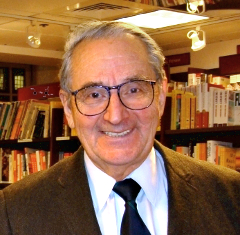
\includegraphics[width=\linewidth]{images/book3/corey.jpg}
\end{minipage}\hfill
\begin{minipage}[t]{0.76\linewidth}
\vspace{0pt}
Les chimistes avaient toujours raisonné à rebours à partir de leurs cibles, mais Elias James Corey, à
partir des années 1960, transforma cette habitude en règles explicites~: la \omterm{def:b2:retrosynthesis:disconnection}{déconnexion}, le \omterm{def:b2:retrosynthesis:disconnection}{synthon}, la
flèche rétrosynthétique, et même des programmes informatiques qui les appliquaient. Il reçut le prix
Nobel de chimie 1990 pour la théorie et la méthodologie de la synthèse organique. (Photographie~: par
Trvthchem, CC0, Wikimedia Commons.)
\end{minipage}
\end{history}

\begin{safety}{\ghs[5mm]{GHS02}\,\ghs[5mm]{GHS03}\,\ghs[5mm]{GHS05}\,\ghs[5mm]{GHS06}\,\ghs[5mm]{GHS07}\,\ghs[5mm]{GHS08}}
Le chlorure d'oxalyle est corrosif, toxique et réagit avec l'eau en libérant du chlorure d'hydrogène~;
l'oxydation de Swern libère du monoxyde de carbone et du sulfure de diméthyle malodorant~: on la conduit
donc sous hotte. Le périodinane de Dess--Martin est un oxydant et ne doit pas être chauffé. On évite
désormais les réactifs du chrome(VI) quand une solution de remplacement existe.
% ledger: ghs:oxalyl-chloride, ghs:DMSO, ghs:DMP
\end{safety}

\section{Exercices}

\begin{exercise}[$\star$]\label{exo:b2:retrosynthesis:1}
Déconnecter chaque alcool en un composé carbonylé et un organomagnésien (donner toutes les possibilités)~:
2-phénylpropan-2-ol, pentan-3-ol, 1-cyclohexyléthanol, 2-méthylbutan-2-ol, 1-phényléthanol.
\end{exercise}

\begin{exercise}[$\star$]\label{exo:b2:retrosynthesis:2}
Pour la \omterm{def:b2:retrosynthesis:disconnection}{déconnexion} du 1-phényléthanol au niveau de la liaison \ce{C-C}, nommer les deux \omterm{def:b2:retrosynthesis:disconnection}{synthons}, dire
lequel est le donneur, et donner un \omterm{def:b2:retrosynthesis:disconnection}{équivalent synthétique} pour chacun.
\end{exercise}

\begin{exercise}[$\star$]\label{exo:b2:retrosynthesis:3}
Une voie en cinq étapes a des rendements par étape de 90, 85, 80, 95 et 70~\%. Calculer son rendement global.
\end{exercise}

\begin{exercise}[$\star$]\label{exo:b2:retrosynthesis:4}
Le 4-oxopentanoate d'éthyle doit être transformé en 5-hydroxypentan-2-one. Planifier la voie avec un
groupe protecteur, et dire pourquoi il est nécessaire.
\end{exercise}

\begin{exercise}[$\star\star$]\label{exo:b2:retrosynthesis:5}
Proposer une rétrosynthèse du butane-1,3-diol à partir de composés d'au plus deux carbones, avec une IGF
et une \omterm{def:b2:retrosynthesis:disconnection}{déconnexion} à deux groupes.
\end{exercise}

\begin{exercise}[$\star\star$]\label{exo:b2:retrosynthesis:6}
Déconnecter la 1-(cyclohex-3-én-1-yl)éthan-1-one par une \omterm{def:b2:frontier-orbitals:diels-alder}{réaction de Diels--Alder}.
\end{exercise}

\begin{exercise}[$\star\star$]\label{exo:b2:retrosynthesis:7}
Déconnecter la 4,4-diméthylcyclohex-2-én-1-one par une \omterm{def:b2:conjugate-additions:robinson}{annélation de Robinson}.
\end{exercise}

\begin{exercise}[$\star\star$]\label{exo:b2:retrosynthesis:8}
La 1-phénylbutan-1-one peut être préparée en une étape par une \omterm{def:b2:aromatic-substitution:friedel-crafts}{acylation de Friedel--Crafts}, ou en deux
à partir du benzaldéhyde. Écrire les deux voies et les comparer.
\end{exercise}

\begin{exercise}[$\star\star$]\label{exo:b2:retrosynthesis:9}
On veut obtenir l'hexanal à partir de l'hexan-1-ol. Quels réactifs le donnent, et lequel donnerait au
contraire l'acide hexanoïque~? Expliquer.
\end{exercise}

\begin{exercise}[$\star\star\star$]\label{exo:b2:retrosynthesis:10}
Dans le 4-aminobutan-1-ol, l'amine doit réagir d'abord avec un \omterm{def:b2:acyl-substitution:derivative}{chlorure d'acyle} lors d'une étape, et
l'alcool plus tard avec un autre. Proposer un couple de \omterm{def:b2:retrosynthesis:orthogonal}{groupes protecteurs orthogonaux} et la séquence.
\end{exercise}

\begin{exercise}[$\star\star\star$]\label{exo:b2:retrosynthesis:11}
Proposer une synthèse de l'hexane-2,5-dione, un composé 1,4-dicarbonylé, à partir du 3-oxobutanoate d'éthyle.
\end{exercise}

\begin{exercise}[$\star\star\star$]\label{exo:b2:retrosynthesis:12}
La 6-méthylhept-5-én-2-one, \ce{(CH3)2C=CHCH2CH2COCH3}, est un intermédiaire de parfumerie. Proposer un
plan complet à partir du 3-oxobutanoate d'éthyle et d'un halogénure~: rétrosynthèse, voie directe, et
l'étape qui élimine l'ester.
\end{exercise}

\section{Problème~: la cétone de framboise}

\begin{problem}[{Problème du week-end --- la rétrosynthèse d'un composé aromatisant, le phénol et
l'opportunité de le protéger, une variante au palladium, et le jugement des voies}]
\label{pb:b2:retrosynthesis:1}
La cétone de framboise, ou 4-(4-hydroxyphényl)butan-2-one, se trouve dans les framboises et d'autres
fruits et sert d'arôme et en parfumerie. Données de l'exercice~: rendements des étapes de la voie
aldolique, 85~\% (condensation) et 92~\% (hydrogénation). Masses molaires (\unit{g/mol})~: C 12.011,
H 1.008, O 15.999, N 14.007, I 126.90. Le $\mathrm pK_a$ du phénol vaut 9.99.
% ledger: use:raspberry-ketone, aw:C, aw:H, aw:O, aw:N, aw:I, pka:phenol, ghs:raspberry-ketone, ghs:4-iodophenol, ghs:MVK

\medskip
\noindent\textbf{Partie I --- Rétrosynthèse.}
\begin{enumerate}
  \item Représenter la cible et nommer ses groupes fonctionnels.
  \item Quelle IGF transforme le motif \ce{ArCH2CH2CO} en un motif doté d'une \omterm{def:b2:retrosynthesis:disconnection}{déconnexion} connue~?
  \item Écrire la cétone insaturée obtenue, avec sa géométrie.
  \item Quel motif à deux groupes contient-elle, et quelle réaction le construit~?
  \item Nommer les deux produits de départ.
  \item Pourquoi cette \omterm{def:b2:enolates-aldol:aldol}{aldolisation} croisée donne-t-elle un seul produit principal~?
  \item Écrire la voie directe en deux étapes, avec les conditions.
\end{enumerate}

\medskip
\noindent\textbf{Partie II --- Le phénol.}
\begin{enumerate}[resume]
  \item Dans l'hydroxyde de sodium aqueux, sous quelle forme se trouve le 4-hydroxybenzaldéhyde~?
        Utiliser le $\mathrm pK_a$.
  \item Comment cette forme modifie-t-elle l'électrophilie de l'aldéhyde~?
  \item Si le phénol était protégé, quel groupe la seconde étape retirerait-elle gratuitement~? Expliquer.
  \item Compter les étapes de la voie avec cette protection.
  \item Le cycle benzénique est-il menacé lors de l'hydrogénation~?
  \item Protéger ou non~? Conclure.
\end{enumerate}

\medskip
\noindent\textbf{Partie III --- Une variante au palladium.}
\begin{enumerate}[resume]
  \item Déconnecter la cétone insaturée au niveau de la liaison entre le cycle et la chaîne~: quels
        partenaires de Heck~?
  \item Écrire la réaction de Heck avec la triéthylamine comme base.
  \item Sur quel carbone de la but-3-én-2-one le groupe aryle se fixe-t-il, et pourquoi~?
  \item Nommer les étapes du \omterm{def:b2:catalytic-cycles:cycle}{cycle catalytique}.
  \item Calculer l'économie d'atomes de l'étape de Heck, en comptant la triéthylamine.
  \item Calculer l'économie d'atomes de la \omterm{def:b2:enolates-aldol:aldol}{crotonisation}.
\end{enumerate}

\medskip
\noindent\textbf{Partie IV --- Juger les voies.}
\begin{enumerate}[resume]
  \item Quelle est l'économie d'atomes de l'hydrogénation~?
  \item Calculer l'économie d'atomes globale de la voie aldolique.
  \item Quelle double liaison l'hydrogénation réduit-elle, et pourquoi la cétone survit-elle~?
  \item Comparer les réactifs des deux voies du point de vue du coût et du danger.
  \item Quelle voie choisir~?
  \item Quel serait l'effet d'une troisième étape à 90~\% sur le rendement global~?
  \item Donner le rendement global de la voie aldolique en deux étapes.
\end{enumerate}
\end{problem}
